\documentclass[a4paper,fleqn]{cas-dc}
\usepackage[numbers]{natbib}

\usepackage{mathtools}
\usepackage{booktabs}
\usepackage{float}
\usepackage{placeins}
\usepackage{flushend}
\usepackage{placeins}
\usepackage{pgfplots}
\pgfplotsset{compat=1.17}
\usepackage{tikz}
\usepackage{float}
\usepackage{graphicx}
\usepackage{graphicx}
\usepackage{algorithm}
\usepackage{algorithmic}
\usepackage{amsmath}
\usepackage{amssymb}  % Add this for \mathbb
\usepackage{tikz}
\usepackage{subcaption}

\numberwithin{equation}{section}
\captionsetup[figure]{font=small,labelfont=bf,justification=centering}
\begin{document}
\let\WriteBookmarks\relax
\def\floatpagepagefraction{1}
\def\textpagefraction{.001}

\shorttitle{Topology-Adaptive Routing under Node Failures in 
Large-Scale Wireless Networks}
\shortauthors{S Gopikrishnan et~al.}

\title [mode = title]{Topology-Adaptive Routing under Node Failures in 
Large-Scale Wireless Networks}      

% Name: A B Reeshma
% Reg No: 23mic7256
% Gmail: abreeshma6002@gmail.com
% vit mail: reeshma.23mic7256@vitapstudent.ac.in
% orcid: 0009-0008-1141-7588


\author[1]{A B Reeshma}[orcid=0009-0008-1141-7588]
\ead{reeshma.23mic7256@vitapstudent.ac.in}
\address[1]{School of Computer Science and Engineering, VIT-AP University, Amaravathi. Andhra Pradesh, India}


\author[2]{A B Reeshma} [orcid=0009-0008-1141-7588]
\cormark[1]
\ead{reeshma.23mic7256@vitapstudent.ac.in}


\author[3]{A B Reeshma} [orcid=0009-0008-1141-7588]
\ead{reeshma.23mic7256@vitapstudent.ac.in}


\cortext[cor1]{Corresponding author}

\begin{abstract}
Large-scale wireless sensor networks are fundamental to modern applications including environmental monitoring, smart infrastructure, disaster management, and Internet of Things based systems. However, these networks face persistent reliability challenges due to node failures caused by energy depletion, hardware degradation, and hostile deployment conditions. Such failures introduce frequent topology changes that result in route breakage, packet loss, and severe degradation of network performance. Existing routing protocols predominantly address energy efficiency or clustering in isolation, without providing the dynamic adaptability needed to maintain reliable communication under node failure conditions. To bridge this gap, this paper proposes the Topology Adaptive Energy-Aware Fault-Tolerant Routing protocol, referred to as TAEFTR, which dynamically reconfigures routing paths in response to real-time network conditions. The proposed protocol integrates continuous node monitoring, energy-threshold-based failure detection, and a multi-metric cost function that simultaneously considers residual energy, inter-node distance, link quality, and traffic load. An energy-aware load balancing mechanism distributes communication traffic across the network to prevent premature node depletion. The protocol is evaluated using the NS-3 network simulator with the AODV protocol as a baseline, with node count varied from 50 to 200 and packet load varied independently. Simulation results demonstrate that TAEFTR maintains stable packet delivery ratios and controlled delay growth under increasing network stress, while achieving improved energy utilization and reduced routing overhead compared to the AODV baseline. The proposed protocol offers a scalable and robust solution for large-scale wireless sensor networks operating under dynamic failure conditions.

\end{abstract}

\begin{keywords}
Wireless Sensor Networks \sep
Fault Tolerant Routing \sep
Topology Adaptive Routing \sep
Energy Efficient Communication \sep
Node Failure Recovery \sep
Load Balancing \sep
NS3 Simulation
\end{keywords}
\maketitle



\section{Introduction}
Modern communication and monitoring systems rely on large-scale wireless sensor networks, currently being used extensively in fields such as environmental monitoring, disaster recovery, smart infrastructure management, and Internet of Things (IoT) implementations. To form these networks, numerous sensor nodes are deployed in a given area and work together to transmit all of their data back to a single sink or base station via multiple hops. Due to their size and decentralized nature, many of the problems experienced in these networks are not sufficiently resolved using traditional networking protocols. An example of this is the unreliable nature of individual sensor nodes in these types of systems. Most sensor nodes are battery operated, with limited capacity, deployed in remote or harsh environments, and are subject to hardware failure due to age over time. This means that node failures happen frequently and without warning. As a result of an individual node failure, routing paths through that node become unusable; leading to failed routes, dropped packets, and in some cases, the complete partitioning of the overall network. As the scale of the network increases, the frequency of node failures also increases making reliable routing an extremely important research topic for this type of network.
This paper addresses the problems posed by Wireless Sensor Network (WSN) in fault tolerance and energy conservation by proposing the Topology-Adaptive Energy-Aware Fault-Tolerant Routing (TAEFTR) protocol, whose implementation and theory are described throughout this research. Specifically, TAEFTR is based on four key principles: It actively monitors the state of every active node (residual energy, link quality, communication responsiveness) on an ongoing basis; it detects node failures quickly (using energy threshold checks and heartbeat timeout); it determines routing paths based on multiple metrics, balancing energy availability, distance, link reliability, and traffic loads; and lastly, it employs load balancing based on remaining energy to provide an even distribution of traffic among nodes while minimizing the likelihood of depleting critical relay nodes. Section 2 will provide a review of related energy-efficient and fault-tolerant routing solutions. Section 3 will formally define the problem addressed by this research. Section 4 will describe TAEFTR's implementation, network model, phases of operation, and mathematical formulations. Section 5 will describe the algorithm design. Section 6 will present simulation results and performance analysis. Finally, Section 7 will summary and discuss ideas for future work.
 

\subsection{Impact of Node Failures in Large-Scale Wireless Networks}

Node failures in large-scale wireless sensor networks arise from multiple interconnected causes. Energy depletion is the most common cause, as nodes continuously consume power for sensing, data processing, and wireless transmission. Once a node's battery falls below a functional threshold, it becomes unable to participate in routing, effectively disappearing from the network topology. Hardware failures, including sensor degradation and communication module malfunctions, also contribute to node loss, particularly in networks deployed in physically demanding environments such as industrial sites or outdoor monitoring fields.
 
The consequences of node failures extend beyond the loss of the failed node itself. Since wireless sensor networks rely on multi-hop routing, the failure of a single intermediate node can sever the only available path between a source region and the base station. In dense networks, this typically triggers a route discovery process that consumes energy and introduces delay. In sparse networks or at network boundaries, the failure may result in unreachable partitions where data cannot be delivered at all. As failures accumulate over the network lifetime, the surviving nodes must take on greater routing loads, accelerating their own energy depletion and creating a cascading failure effect.
\subsection{Research Objectives}

This research pursues four primary objectives. The first objective is to develop a comprehensive understanding of how node failures affect routing performance in large-scale wireless sensor networks, with particular focus on the relationship between failure frequency, topology instability, and degradation of key performance metrics including packet delivery ratio, delay, throughput, and energy consumption.
 
The second objective is to design a fault-tolerant routing mechanism that detects node failures in real time and dynamically reconfigures routing paths to maintain uninterrupted data delivery. This mechanism must operate in a distributed manner without requiring global knowledge of network state, making it scalable to large network sizes.
 
The third objective is to develop a routing cost function that integrates multiple network parameters, specifically residual energy, inter-node distance, link quality, and traffic load, into a unified decision criterion. This multi-metric approach enables the protocol to make routing decisions that balance energy efficiency, communication reliability, and congestion avoidance simultaneously rather than optimizing a single metric at the expense of others.
 
The fourth objective is to validate the proposed protocol through systematic simulation experiments and compare its performance against the AODV baseline routing protocol. The evaluation measures packet delivery ratio, end-to-end delay, throughput, energy consumption, communication overhead, and jitter across varying network sizes and traffic loads.

\section{Literature Survey}

This section reviews existing research related to routing optimization, energy efficiency, and fault tolerance in wireless sensor networks. A large number of routing protocols have been proposed to improve network lifetime, reduce communication overhead, and enhance reliable data delivery under resource constrained conditions. Most existing methods focus on clustering, metaheuristic optimization, intelligent sink placement, or adaptive route selection to minimize energy dissipation. Recent studies also address dynamic network challenges such as node mobility, link breakage, congestion, and topology variation. Several protocols incorporate machine learning, fuzzy logic, swarm intelligence, and reinforcement learning to improve routing decisions under changing network conditions. Although these approaches achieve improvements in specific performance metrics, many of them optimize only one or two objectives and do not simultaneously address energy balancing, failure recovery, scalability, and topology adaptation. To better understand the current research landscape, the literature is grouped into two major categories. The first category focuses on energy-efficient routing approaches designed to extend network lifetime through optimized communication and clustering strategies. The second category covers fault-tolerant and failure-aware routing techniques that aim to maintain connectivity and reliable packet delivery during node or link failures. The review highlights the strengths and limitations of existing methods and motivates the need for the proposed Topology Adaptive Energy Aware Fault Tolerant Routing protocol.
\subsection{Energy-Efficient Routing Approaches}

Research on energy-efficient routing for wireless sensor networks has been extensive, with multiple approaches proposed to extend network lifetime through intelligent resource management. Gururaj et al.~\cite{gururaj2023collaborative} proposed a collaborative energy-efficient routing protocol for 5G and 6G wireless sensor network communication, incorporating a reinforcement learning algorithm for cluster group formation and a residual energy based cluster head selection method. Wang et al.~\cite{wang2024energy} employed fuzzy c-means clustering combined with quantum annealing to optimize energy consumption, incorporating residual energy, neighbor count, distance to base station, and node centrality as decision parameters.
 
Marine and underwater sensor network environments present additional routing challenges due to high path loss and mobility. Hussain et al.~\cite{hussain2023cr} addressed these challenges through a cooperative relay optimization scheme offering energy-efficient, path-loss-aware routing for underwater wireless sensor networks. Vellaichamy et al.~\cite{vellaichamy2023wireless} applied the moth flame and salp swarm optimization algorithms for multi-criteria clustering and energy-efficient routing in terrestrial sensor networks. Hemanand et al.~\cite{hemanand2023analysis} analyzed the effects of mobility, static sink relocation, and multiple sink configurations on sensor network longevity, demonstrating that intelligent sink placement can significantly reduce energy dissipation.
 
Barnwal et al.~\cite{barnwal2023improved} developed the MHCRT-EEWSN algorithm combining the Weighted Modified Flamingo Optimization algorithm for cluster head selection and the Improved Artificial Bee Optimization algorithm for route selection using multi-parameter fitness functions. Sah et al.~\cite{sah2023efficient} proposed the ERAS cluster-based routing technique addressing the energy scarcity problem through TDMA-based scheduling to prevent inter-cluster message collisions.

\subsection{Fault-Tolerant and Failure-Aware Routing Techniques}
Fault tolerance in wireless sensor networks has been approached through a variety of mechanisms. Pedditi and Debasis~\cite{pedditi2023energy} proposed an energy-efficient TDMA-based routing protocol for IoT wireless sensor networks used in forest fire detection, incorporating event-driven reporting to minimize redundant transmissions and preventing low-energy nodes from assuming cluster head roles. Gupta et al.~\cite{gupta2024optimizing} proposed mesh topology optimization using ant colony-based bio-inspired techniques for varying sensor densities.
 
Manhar and Dembla~\cite{manhar2023improved} addressed the abrupt link failure problem in mobile ad hoc networks by developing an improved hybrid routing protocol that integrates multiple routing strategies. Foko et al.~\cite{foko2024arpmec} proposed an adaptive routing protocol for IoT networks based on Mobile Edge Computing, where cluster heads are elected based on link quality and clusters communicate through MEC servers to maintain connectivity under mobility. Moussa et al.~\cite{moussa2023novel} developed an energy-efficient and reliable routing protocol combining optimized clustering with an ant colony optimization based data transmission algorithm.
 
Liu and Guo~\cite{liu2023mmscm} presented a hierarchical routing protocol for mobile wireless sensor networks using multiple mobile sinks. Zou et al.~\cite{zou2024survey} provided a comprehensive survey of fault-tolerant consensus mechanisms in wireless networks covering both Byzantine and non-Byzantine fault models. LT and LF~\cite{lt2023energy} developed the SExpNMA meta-heuristic algorithm combining Newton's Method Algorithm and serial Exponential Weighted Moving Average for fault-tolerant routing in agricultural wireless sensor networks.

\begin{table*}[ht]
\centering
\caption{Literature Survey Summary}
\renewcommand{\arraystretch}{1.3}
\resizebox{\textwidth}{!}{%
\begin{tabular}{|c|p{3.2cm}|p{3.5cm}|p{3.8cm}|p{3.8cm}|}
\hline
\textbf{Ref} & \textbf{Method Proposed} & \textbf{Techniques Used} & \textbf{Issues Resolved} & \textbf{Limitations} \\
\hline

R3 & Priority-based routing for UWSNs \cite{ismail2023novel} 
& Energy and priority-aware forwarding mechanism 
& Improves packet delivery and reduces energy consumption 
& Limited scalability and weak adaptability under topology changes \\
\hline

R4 & Secure cluster-based routing for WBANs \cite{dass2023cluster} 
& Clustering with secure optimal path selection 
& Enhances data integrity and communication reliability 
& Limited fault tolerance under frequent node failures \\
\hline

R13 & MOORP opportunistic routing protocol \cite{chaurasia2023moorp} 
& Dragonfly metaheuristic and forwarder selection strategy 
& Improves energy efficiency and packet delivery ratio 
& Higher computation overhead and limited topology awareness \\
\hline

R14 & GAN-based trusted routing (GTR) for UWSNs \cite{wang2024gtr} 
& Trust evaluation using GAN and Q-learning 
& Improves security and malicious node detection accuracy 
& High computational complexity and energy overhead \\
\hline

R20 & Secure energy-efficient routing protocol \cite{pragadeswaran2024energy} 
& Homomorphic encryption-based secure routing 
& Enhances data confidentiality and network security 
& Increased processing overhead and reduced adaptability \\
\hline

R21 & Accuracy-aware energy-efficient multipath routing algorithm \cite{dan2024accuracy} 
& Artificial immune algorithm, multi-objective optimization 
& Improves data accuracy and transmission reliability under interference 
& Increased computational complexity and limited adaptability to dynamic node failures \\
\hline

R22 & Secure routing protocol for industrial WSN applications \cite{onyema2025secure} 
& Machine learning, MCDM-based clustering and routing 
& Enhances security, reduces data loss, and improves energy efficiency 
& High overhead due to security computation and limited scalability analysis \\
\hline

R23 & Local density-aware opportunistic routing protocol (FCM-OR) \cite{lata2025fcm} 
& Fuzzy c-means clustering, opportunistic routing 
& Improves forwarding efficiency in dense and non-uniform networks 
& Broadcast redundancy and lack of topology recovery under node failures \\
\hline

R24 & LEACH-based energy-efficient routing enhancements \cite{siamantas2025energy} 
& Hierarchical clustering, sleep--awake scheduling 
& Extends network lifetime and reduces energy consumption 
& Cluster-head failure handling is limited and topology adaptation is weak \\
\hline

R25 & Comprehensive review of energy-efficient routing protocols \cite{bekal2024comprehensive} 
& Comparative analysis of standard and enhanced routing schemes 
& Identifies energy efficiency challenges and protocol trade-offs 
& Does not propose adaptive routing or fault-tolerant solutions \\
\hline

R26 & Reliability and availability assessment model for WSNs \cite{heidari2024assessment} 
& Fault tree analysis, Markov chain modeling 
& Evaluates network reliability under permanent node faults 
& Focuses on evaluation only, without providing routing adaptation mechanisms \\
\hline

R27 & Grid-based routing taxonomy for WSNs \cite{jain2024taxonomy} 
& Virtual grid topology, hierarchical routing analysis 
& Improves scalability and energy balance in large-scale networks 
& Grid header failure causes performance degradation \\
\hline

R28 & Survey on routing protocols for WBANs \cite{goyal2023routing} 
& Classification-based comparative analysis 
& Highlights energy, QoS, and mobility challenges 
& Application-specific and not suitable for large-scale WSNs \\
\hline

R29 & Energy-efficient routing review for underwater WSNs \cite{khan2024energy} 
& Taxonomy-based comparison, ML-assisted routing analysis 
& Identifies adaptive and intelligent routing requirements 
& Environment-specific and limited applicability to terrestrial networks \\
\hline

R30 & Secure and Energy-Efficient Routing for Industrial IoT \cite{othman2023multi} 
& Machine learning-based routing and security framework 
& Enhances reliability and energy efficiency under industrial conditions 
& Increased complexity and limited topology-adaptive fault handling \\
\hline

\end{tabular}%
}
\end{table*}
\clearpage
\subsection{Research Gap and Motivation}
Analysis of the existing literature reveals a consistent pattern: most routing protocols are optimized for a single concern such as energy efficiency, clustering quality, or security, while providing only limited support for dynamic topology adaptation under node failure conditions. Many approaches depend on static routing structures or infrequent topology updates, which are unsuitable for the continuous topology changes characteristic of large-scale wireless sensor networks experiencing node failures.
 
Specifically, protocols that achieve strong energy efficiency often rely on pre-established cluster structures that break down when cluster heads fail. Security-focused protocols introduce computational overhead that accelerates energy depletion. Opportunistic routing protocols improve delivery ratios but lack mechanisms for recovering from topology disruptions. No reviewed protocol simultaneously addresses real-time failure detection, dynamic path reconfiguration, multi-metric routing optimization, and energy-aware load balancing within a unified framework.
 
This gap motivates the design of TAEFTR, a protocol that treats topology adaptation as its primary design objective while incorporating energy awareness, fault tolerance, and load balancing as integral components rather than secondary considerations.

\section{Problem Statement}
 Large-scale wireless sensor networks are often deployed in environments where node failures occur frequently due to energy depletion, harsh environmental conditions, and hardware degradation. Therefore, routing in such networks must be adaptive, reliable, and energy-efficient.  

Given a network of $N$ sensor nodes distributed over a sensing region, where nodes may fail at any time because of battery exhaustion or communication loss, the objective is to design a routing protocol $\mathcal{P}$ that can rapidly detect node failures within a bounded response time $\tau$ without centralized coordination. The protocol should dynamically reconstruct routing paths after each detected failure so that continuous data delivery to the base station is maintained. It must also select routes by minimizing a multi-metric cost function based on residual energy, communication distance, link quality, and traffic load. In addition, the protocol should balance communication load among nodes to avoid early depletion of important relay nodes and thereby extend overall network lifetime. Finally, the protocol must remain scalable for large networks while keeping communication overhead low.  

Existing routing protocols address only some of these requirements. Static or pre-computed routing methods are weak in failure detection and route recovery. Single-metric optimization techniques cannot achieve balanced route selection. Load-unaware protocols cause uneven energy consumption, while centralized approaches suffer from scalability limitations. To overcome these challenges, the proposed TAEFTR protocol integrates continuous monitoring, fast failure detection, adaptive cost-based routing, and energy-aware load balancing in a unified framework.


\section{Proposed Work}
The proposed Topology Adaptive Energy-Aware Fault-Tolerant Routing protocol, referred to as TAEFTR, is designed to provide reliable and efficient communication in large-scale wireless sensor networks under dynamic node failure conditions. The protocol integrates continuous node monitoring, energy-based failure detection, multi-metric adaptive routing, and energy-aware load balancing into a unified operational framework.
\subsection{Network Model}

In this research work, a large-scale Wireless Sensor Network (WSN) composed of $N$ sensor nodes is considered. These sensor nodes are randomly deployed over a two-dimensional sensing region of size $A = L \times W$, where $L$ and $W$ represent the length and width of the monitoring area, respectively. Random deployment is appropriate for real-time applications such as environmental monitoring, forest fire detection, military surveillance, smart agriculture, and disaster management, where manual placement of nodes is either costly or impractical.

Each sensor node is equipped with sensing, processing, storage, and wireless communication capabilities. The network operates in a distributed and self-organized manner, where nodes cooperate with neighboring nodes to forward sensed information toward the base station using multi-hop communication. Let the complete set of deployed nodes be denoted as

\begin{equation}
\mathcal{N} = \{n_1, n_2, \ldots, n_N\},
\end{equation}

where each node $n_i$ is represented by its geographical coordinates $(x_i, y_i)$. The base station is assumed to have higher computational power and sufficient energy resources compared to normal sensor nodes.

\subsubsection{Distance Model}

Communication between sensor nodes strongly depends on their physical separation. The Euclidean distance between two nodes $n_i$ and $n_j$ is calculated as

\begin{equation}
\label{eq:dist}
d_{ij} = \sqrt{(x_i - x_j)^2 + (y_i - y_j)^2}
\end{equation}

A direct wireless communication link between two nodes exists only if

\begin{equation}
d_{ij} \leq R
\end{equation}

where $R$ denotes the maximum communication range of a sensor node. Nodes located outside this range must communicate through intermediate relay nodes. This distance constraint reduces unnecessary transmission power and improves energy efficiency throughout the network.

\subsubsection{Graph Representation}

The wireless sensor network can be represented as an undirected graph $G = (V,E)$, where $V$ denotes the set of deployed sensor nodes and $E$ denotes the set of available communication links. An edge $(n_i,n_j)$ exists whenever the condition $d_{ij} \leq R$ is satisfied. This graph model is useful for analyzing network connectivity, shortest paths, fault recovery, and route optimization.

\subsubsection{Energy Model}

Energy is the most valuable resource in wireless sensor networks because sensor nodes usually operate on limited battery power. Recharging or replacing batteries may not be possible after deployment. Therefore, efficient energy utilization is essential for prolonging network lifetime.

Each node is initialized with energy $E_0$. The energy consumed to transmit a $k$-bit packet over distance $d$ is given by

\begin{equation}
\label{eq:etx}
E_{tx}(k,d)=kE_{elec}+k\epsilon_{amp}d^{\eta}
\end{equation}

where $E_{elec}$ is the energy required for electronic circuitry, $\epsilon_{amp}$ is the amplifier coefficient, and $\eta$ is the path-loss exponent.

The energy consumed for receiving a $k$-bit packet is

\begin{equation}
\label{eq:erx}
E_{rx}(k)=kE_{elec}
\end{equation}

The residual energy of node $n_i$ at time instant $t$ is updated as

\begin{equation}
\label{eq:residual}
E_i(t)=E_i(t-1)-E_{used}(t)
\end{equation}

where $E_{used}(t)$ is the total energy consumed for transmission, reception, and local processing during time interval $t$.

A node is considered inactive when its remaining energy falls below the threshold level:

\begin{equation}
\label{eq:dead}
E_i(t)\leq E_{th}
\end{equation}

Proper energy management helps maintain network connectivity and delays node failures.

\subsubsection{Link Quality Model}

Reliable communication depends on both distance and signal conditions. The link quality between nodes $n_i$ and $n_j$ is estimated as

\begin{equation}
\label{eq:lq}
LQ_{ij}=\frac{RSSI_{ij}}{d_{ij}}
\end{equation}

where $RSSI_{ij}$ represents the received signal strength indicator. Higher values of $LQ_{ij}$ indicate stronger, more stable, and reliable wireless links. Selecting links with better quality reduces retransmissions, delay, and packet loss.

\subsubsection{Routing Cost Function}

To identify the best next-hop node, a multi-parameter routing cost function is defined as

\begin{equation}
\label{eq:cost}
C_{ij}=
\alpha \frac{1}{E_j}
+\beta d_{ij}
+\gamma \frac{1}{LQ_{ij}}
+\delta T_j
\end{equation}

where $E_j$ is the residual energy of node $j$, $d_{ij}$ is the distance between nodes $i$ and $j$, $LQ_{ij}$ is the measured link quality, and $T_j$ is the current traffic load of node $j$. The weighting parameters $\alpha$, $\beta$, $\gamma$, and $\delta$ determine the importance of each metric according to network requirements.

This cost formulation ensures that nodes with higher residual energy, shorter communication distance, better link quality, and lower traffic congestion receive lower routing cost values and are therefore selected as forwarding nodes.

\subsubsection{Routing Decision Metrics}

Table~\ref{tab:decision_metrics} presents the important metrics used in routing decisions. Considering multiple metrics simultaneously enables the proposed protocol to achieve balanced optimization between network lifetime, communication reliability, throughput, and delay.
\begin{table*}[ht]
\centering
\caption{Routing Decision Metrics and Their Impact in TAEFTR}
\label{tab:decision_metrics}
\renewcommand{\arraystretch}{1.4}
\resizebox{\textwidth}{!}{%
\begin{tabular}{|c|p{4cm}|p{8.5cm}|}
\hline
\textbf{Metric} & \textbf{Description} & \textbf{Impact on Routing Decision} \\
\hline

Residual Energy ($E_j$) 
& Remaining battery power of node $j$ 
& Nodes with higher energy are preferred to avoid premature node failure and extend network lifetime. \\
\hline

Distance ($d_{ij}$) 
& Euclidean distance between nodes $i$ and $j$ 
& Shorter distance lowers transmission energy consumption and improves communication efficiency. \\
\hline

Link Quality ($LQ_{ij}$) 
& Stability and strength of communication link 
& Better links reduce packet loss, retransmissions, and transmission delay. \\
\hline

Traffic Load ($T_j$) 
& Current communication burden on node $j$ 
& Lower traffic load prevents congestion and improves packet delivery performance. \\
\hline

Weight Parameters ($\alpha,\beta,\gamma,\delta$) 
& Relative importance of routing metrics 
& Proper tuning balances energy efficiency, reliability, throughput, and network lifetime. \\
\hline

\end{tabular}%
}
\end{table*}

\subsubsection{Node Failure Model}

Node failures are common in large-scale WSNs due to battery depletion, hardware damage, interference, or communication loss. A node is considered failed when

\begin{equation}
\label{eq:failure}
F_i=
\begin{cases}
1, & E_i(t)\leq E_{th} \\
1, & \text{heartbeat timeout occurs} \\
0, & \text{otherwise}
\end{cases}
\end{equation}

where $F_i=1$ denotes a failed node and $F_i=0$ denotes an active node.

Once a node is marked as failed, it is immediately removed from neighbor tables and excluded from future routing decisions. This enables the routing protocol to rapidly adapt to topology changes and continue packet forwarding through alternate paths.

Overall, the proposed network model provides a strong theoretical and practical foundation for the Topology Adaptive Energy-Aware Fault-Tolerant Routing (TAEFTR) protocol by jointly considering distance, energy efficiency, communication reliability, traffic balancing, and fault tolerance.

\subsection{Overview}

The overall workflow of the proposed Topology Adaptive Energy-Aware Fault-Tolerant Routing (TAEFTR) protocol is illustrated in Fig.~\ref{fig:overview}. The operation begins with wireless sensor network initialization, where sensor nodes are randomly deployed in the sensing area and assigned initial energy levels. During this phase, neighboring nodes are identified and basic network connectivity is established.

After initialization, the protocol continuously monitors important node parameters such as residual energy, link quality, and neighbor availability in order to maintain an updated view of network conditions. This monitoring process enables the protocol to quickly identify topology changes and communication issues.
\begin{figure*}[!t]
\centering
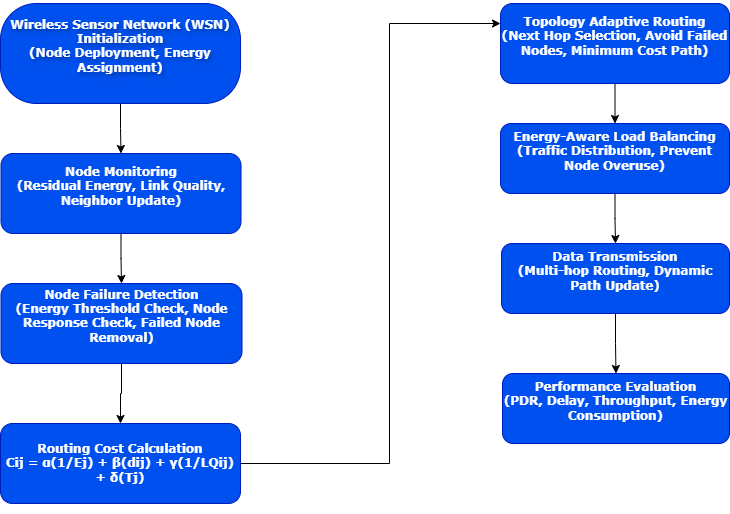
\includegraphics[width=0.75\textwidth]{figures/overview-fig.drawio.png}
\caption{Overall workflow of the proposed TAEFTR protocol showing network initialization, node monitoring, failure detection, cost-based routing, topology adaptation, load balancing, data transmission, and performance evaluation.}
\label{fig:overview}
\end{figure*}

When abnormal conditions are detected, the protocol performs node failure detection using residual energy threshold analysis and node response verification. Failed or inactive nodes are immediately excluded from routing decisions to avoid packet loss and route interruption.

Next, the routing cost of candidate forwarding nodes is computed using multiple parameters including residual energy, communication distance, link quality, and traffic load. Based on the minimum routing cost, the protocol dynamically selects the most suitable next-hop node and reconstructs routes whenever failures occur.

To improve network lifetime, an energy-aware load balancing mechanism distributes traffic across multiple nodes and prevents excessive burden on specific relay nodes. Finally, sensed data is transmitted to the base station through adaptive multi-hop communication paths. The overall performance of the proposed protocol is evaluated using packet delivery ratio, end-to-end delay, throughput, and total energy consumption.
\subsection{Phase 1: Network Initialization}

In the first operational phase, a large number of sensor nodes are randomly deployed throughout the sensing region. The sensing area is represented as $A=L \times W$, where $L$ and $W$ denote the length and width of the monitoring field, respectively. Random deployment is suitable for practical environments such as forest monitoring, military surveillance, industrial sensing, and disaster recovery operations, where planned node placement is difficult.

Each deployed node is assigned a unique identifier and an initial energy value $E_0$. The position of node $n_i$ is represented by coordinates $(x_i,y_i)$. Based on the deployment, each node identifies neighboring nodes that lie within communication range $R$. The Euclidean distance between any two nodes $n_i$ and $n_j$ is calculated using (\ref{eq:dist}):

\begin{equation}
d_{ij}=\sqrt{(x_i-x_j)^2+(y_i-y_j)^2}
\end{equation}

A direct communication link is established only when

\begin{equation}
d_{ij}\leq R
\end{equation}

Thus, the initial network topology is formed by discovering all reachable neighboring nodes. Each node creates a local neighbor table storing node identity, residual energy, distance, link quality, and active status. This initialization stage provides the basic framework for all future routing and monitoring operations.

\subsection{Phase 2: Neighbor Discovery and Monitoring}

After initialization, each node continuously performs neighbor discovery and network monitoring. Periodic control packets or heartbeat messages are exchanged among neighboring nodes to maintain updated connectivity information.

The neighbor set of node $n_i$ is defined as

\begin{equation}
\label{eq:neighbor}
N_i=\{n_j \mid d_{ij}\leq R\}
\end{equation}

where only nodes satisfying the communication range condition are considered valid neighbors.

The degree of node $n_i$, which indicates the number of neighboring nodes, is expressed as

\begin{equation}
Deg(n_i)=|N_i|
\end{equation}

A larger node degree generally improves connectivity and route availability.

During monitoring, each node periodically updates:

\begin{itemize}
\item Residual energy of neighbors
\item Link quality values
\item Response status of neighboring nodes
\item Current traffic load
\end{itemize}

The monitoring interval is represented as $\Delta t$, and status information is refreshed after every interval. This continuous observation allows the network to quickly react to changing topology and communication conditions.

\subsection{Phase 3: Node Failure Detection}

Node failure is a common event in large-scale WSNs due to battery exhaustion, hardware malfunction, environmental damage, or communication loss. Therefore, the proposed TAEFTR protocol incorporates an efficient node failure detection mechanism.

A node is considered failed if its residual energy becomes lower than threshold $E_{th}$ or if it does not respond within a predefined heartbeat timeout interval.

The failure model is defined as

\begin{equation}
\label{eq:failure_proposed}
F_i=
\begin{cases}
1, & E_i(t)\leq E_{th} \\
1, & \text{heartbeat timeout} \\
0, & \text{otherwise}
\end{cases}
\end{equation}

where:

\begin{itemize}
\item $F_i=1$ indicates failed node
\item $F_i=0$ indicates active node
\end{itemize}

The heartbeat timeout can be represented as

\begin{equation}
T_{resp}>T_{max}
\end{equation}

where $T_{resp}$ is node response time and $T_{max}$ is maximum allowed delay.

Once a node is marked failed, it is removed from neighbor tables:

\begin{equation}
N_j=N_j-\{n_i\}
\end{equation}

for all neighboring nodes $n_j$. This prevents the failed node from participating in future routing operations.

\subsection{Phase 4: Topology-Adaptive Routing}

The routing process in TAEFTR dynamically adapts to topology changes caused by node failures or energy depletion. Instead of relying on fixed paths, the next-hop node is selected in real time using a multi-metric routing cost function.

The routing cost between node $n_i$ and candidate node $n_j$ is defined as

\begin{equation}
\label{eq:cost_proposed}
C_{ij}=
\alpha \frac{1}{E_j}
+\beta d_{ij}
+\gamma \frac{1}{LQ_{ij}}
+\delta T_j
\end{equation}

where:

\begin{itemize}
\item $E_j$ = residual energy of node $j$
\item $d_{ij}$ = distance between nodes $i$ and $j$
\item $LQ_{ij}$ = link quality
\item $T_j$ = traffic load of node $j$
\item $\alpha,\beta,\gamma,\delta$ = weighting factors
\end{itemize}

The selected next-hop node is

\begin{equation}
\label{eq:nexthop}
NextHop=\arg\min_{n_j \in N_i}(C_{ij})
\end{equation}

Thus, nodes with higher energy, lower traffic, better link quality, and shorter distance are preferred.
As shown in Fig.~\ref{fig:fault_recovery}, the proposed routing protocol detects failed nodes and immediately selects an alternate communication path.

\begin{figure*}[!t]
\centering
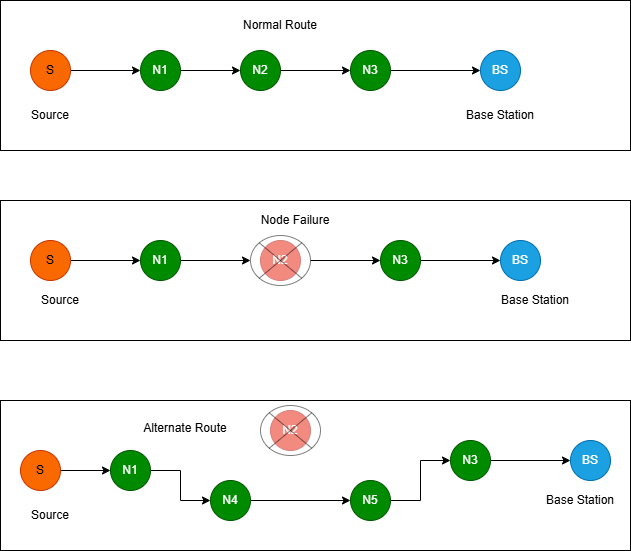
\includegraphics[width=0.75\textwidth]{figures/second-fig.drawio.png}
\caption{Dynamic fault recovery mechanism in the proposed TAEFTR protocol showing normal routing, node failure detection, and alternate path reconstruction.}
\label{fig:fault_recovery}
\end{figure*}

\begin{equation}
Path = \{S,n_1,n_2,\dots,BS\}
\end{equation}

If any intermediate node fails, a new path is recalculated immediately.

\subsection{Phase 5: Energy-Aware Load Balancing}

To avoid overuse of frequently selected relay nodes, TAEFTR incorporates an energy-aware load balancing mechanism. This prevents premature energy exhaustion and improves network lifetime.

The load balancing factor is defined as

\begin{equation}
\label{eq:lb}
LB_i=\frac{T_i}{E_i}
\end{equation}

where:

\begin{itemize}
\item $T_i$ = current traffic load
\item $E_i$ = residual energy
\end{itemize}

A lower $LB_i$ value indicates a more suitable forwarding node.

Traffic can be redistributed according to

\begin{equation}
T_i^{new}=T_i-\Delta T,\quad T_j^{new}=T_j+\Delta T
\end{equation}

where $\Delta T$ is the shifted traffic load from overloaded node $i$ to alternate node $j$.

This mechanism balances packet forwarding responsibility across multiple nodes and prevents traffic bottlenecks.

\subsection{Phase 6: Data Transmission and Adaptation}

After route selection, sensed packets are transmitted toward the base station through dynamically selected multi-hop paths. Suppose source node $S$ generates packet $P_k$. Then transmission occurs as

\begin{equation}
S \rightarrow n_1 \rightarrow n_2 \rightarrow \cdots \rightarrow BS
\end{equation}

At each hop, the forwarding node recalculates the next-hop using (\ref{eq:nexthop}) based on current network state.

The packet delivery ratio is expressed as

\begin{equation}
PDR=\frac{P_{recv}}{P_{sent}}\times 100
\end{equation}

The average delay is

\begin{equation}
Delay=\frac{\sum (t_{recv}-t_{sent})}{N_p}
\end{equation}

The throughput is

\begin{equation}
Throughput=\frac{Total\ Bits\ Received}{Simulation\ Time}
\end{equation}

Total consumed energy is

\begin{equation}
E_{total}=\sum_{i=1}^{N}(E_0-E_i)
\end{equation}

If a selected node fails during active transmission, the protocol immediately computes an alternate next-hop node and resumes forwarding without restarting the entire route discovery process.

Overall, the proposed methodology effectively integrates node initialization, continuous monitoring, failure detection, topology-adaptive routing, energy-aware load balancing, and reliable data transmission. By utilizing the mathematical formulations from (\ref{eq:neighbor}) to (\ref{eq:lb}), the TAEFTR protocol achieves improved packet delivery, lower delay, balanced energy consumption, and enhanced scalability in large-scale wireless sensor networks.
\section{Algorithm Design}

The proposed Topology Adaptive Energy-Aware Fault-Tolerant Routing (TAEFTR) algorithm is developed to provide reliable, scalable, and energy-efficient communication in large-scale wireless sensor networks operating under dynamic topology conditions. In practical sensor deployments, node failures occur frequently due to battery depletion, environmental effects, communication loss, or hardware degradation. Therefore, the routing mechanism must continuously adapt itself to maintain stable data transmission.

Unlike conventional static routing approaches, the proposed algorithm updates forwarding decisions in real time according to residual energy, communication distance, link quality, and traffic load. Whenever a node becomes unavailable, the protocol immediately reconstructs an alternate route without requiring complete network rediscovery. This significantly reduces packet loss and communication delay.

The TAEFTR framework is divided into three major operational components: (i) continuous node monitoring and failure detection, (ii) adaptive next-hop selection using a multi-metric routing function, and (iii) energy-aware load balancing to improve network lifetime. These components work together to provide robust communication in large-scale wireless sensor networks.

The major parameters used in the proposed algorithm are summarized in Table~\ref{tab:params}.

\begin{table}[h]
\centering
\caption{Parameters Used in TAEFTR Algorithm}
\label{tab:params}
\renewcommand{\arraystretch}{1.2}
\begin{tabular}{|c|p{6cm}|}
\hline
\textbf{Symbol} & \textbf{Description} \\
\hline
$N$ & Set of deployed sensor nodes \\
$BS$ & Base station \\
$E_i$ & Residual energy of node $i$ \\
$E_{th}$ & Threshold energy below which node is inactive \\
$d_{ij}$ & Distance between nodes $i$ and $j$ \\
$LQ_{ij}$ & Link quality between nodes $i$ and $j$ \\
$T_j$ & Traffic load of node $j$ \\
$C_{ij}$ & Routing cost value \\
$F_i$ & Failure status of node $i$ \\
$NextHop$ & Selected forwarding node \\
$R$ & Communication range \\
\hline
\end{tabular}
\end{table}

The routing cost function used in forwarding decisions is defined as

\begin{equation}
C_{ij}=
\alpha \frac{1}{E_j}
+\beta d_{ij}
+\gamma \frac{1}{LQ_{ij}}
+\delta T_j
\end{equation}

where $\alpha,\beta,\gamma,\delta$ are weighting coefficients. Lower cost values indicate better forwarding nodes.

%=========================================================
\begin{algorithm}[!ht]
\caption{Algorithm 1: TAEFTR Main Routing Procedure}
\label{alg:main}
\begin{algorithmic}[1]

\STATE Deploy $N$ sensor nodes randomly in sensing region
\STATE Assign initial energy $E_0$ to every node
\STATE Initialize node coordinates and communication radius $R$
\STATE Discover neighboring nodes for all deployed nodes
\STATE Construct local neighbor tables
\STATE Initialize routing status and traffic counters

\WHILE{network remains operational}

    \STATE Update topology information periodically
    \STATE Execute FailureDetection()

    \FOR{each source node requesting packet transmission}

        \STATE Retrieve current neighbor list
        \STATE Execute SelectNextHop()

        \IF{$NextHop \neq NULL$}

            \STATE Forward packet to selected next-hop node
            \STATE Deduct transmission energy from sender
            \STATE Deduct reception energy from receiver
            \STATE Update traffic counter of selected node
            \STATE Continue forwarding until base station reached

        \ELSE

            \STATE Store packet temporarily
            \STATE Wait for topology recovery

        \ENDIF

    \ENDFOR

    \STATE Execute LoadBalancing()
    \STATE Update total consumed energy
    \STATE Measure throughput and packet delivery ratio

\ENDWHILE

\STATE Generate final network statistics

\end{algorithmic}
\end{algorithm}
\subsection{Algorithm 2: Node Failure Detection}

The node failure detection component is one of the most important modules of the proposed TAEFTR protocol because routing reliability directly depends on the availability of active forwarding nodes. In large-scale wireless sensor networks, node failures are common due to battery depletion, hardware damage, signal interference, harsh environmental conditions, or communication breakdown. If failed nodes are not identified quickly, packets may continue to be forwarded through invalid routes, resulting in retransmissions, packet loss, increased delay, and unnecessary energy consumption.

To address this problem, the proposed method continuously monitors the operational condition of every node using two major indicators: residual energy and communication responsiveness. The residual energy of node $n_i$ at time instant $t$ is represented as

\begin{equation}
E_i(t)=E_i(t-1)-E_{used}(t)
\end{equation}

where $E_{used}(t)$ denotes the energy consumed for sensing, processing, transmission, and reception during the current interval.

A node is considered failed when its energy falls below the threshold level $E_{th}$ or when heartbeat signals are not received within the predefined timeout duration. The failure decision is mathematically expressed as

\begin{equation}
F_i=
\begin{cases}
1, & E_i(t)\leq E_{th} \\
1, & T_{resp}>T_{max} \\
0, & \text{otherwise}
\end{cases}
\end{equation}

where $F_i=1$ indicates node failure, $T_{resp}$ is node response time, and $T_{max}$ is the maximum acceptable response interval.

Once a node is marked as failed, it is immediately removed from routing tables and neighboring node lists. This proactive detection process enables the network to reconstruct routes quickly and maintain stable communication performance.

\begin{algorithm}[H]
\caption{Algorithm 2: FailureDetection()}
\label{alg:fault}
\begin{algorithmic}[1]

\FOR{each node $n_i \in N$}

    \STATE Read current residual energy $E_i$
    \STATE Check heartbeat response status
    \STATE Measure response delay

    \IF{$E_i \leq E_{th}$}

        \STATE $F_i \leftarrow 1$
        \STATE Mark node failed due to low energy

    \ELSIF{$T_{resp} > T_{max}$}

        \STATE $F_i \leftarrow 1$
        \STATE Mark node failed due to timeout

    \ELSE

        \STATE $F_i \leftarrow 0$

    \ENDIF

    \IF{$F_i = 1$}

        \STATE Remove $n_i$ from neighbor tables
        \STATE Remove $n_i$ from routing paths
        \STATE Trigger route recovery

    \ENDIF

\ENDFOR

\end{algorithmic}
\end{algorithm}

%=========================================================
\subsection{Algorithm 3: Adaptive Next Hop Selection with Energy Aware Load Balancing}

The proposed TAEFTR protocol combines next hop selection and load balancing into a unified decision process. Instead of selecting a forwarding node based only on shortest path distance, the method jointly considers residual energy, communication distance, link quality, and current traffic load. This integrated strategy improves route stability, avoids congested relay nodes, and prolongs network lifetime.

For a transmitting node $n_i$, each active neighboring node $n_j$ is evaluated using the routing cost function

\begin{equation}
\label{eq:combined_cost}
C_{ij}=
\alpha \frac{1}{E_j}
+\beta d_{ij}
+\gamma \frac{1}{LQ_{ij}}
+\delta T_j
\end{equation}

where $E_j$ represents residual energy, $d_{ij}$ denotes communication distance, $LQ_{ij}$ is link quality, and $T_j$ is the traffic load of candidate node $n_j$. The weighting coefficients $\alpha,\beta,\gamma,\delta$ control the contribution of each metric.

The communication burden of a node is further represented by the load balancing factor

\begin{equation}
\label{eq:lb_factor}
LB_j=\frac{T_j}{E_j}
\end{equation}

Nodes with lower load factor values are preferred because they have smaller traffic burden and higher remaining energy. If the selected node becomes overloaded, part of the traffic is shifted to another neighboring node with lower cost.

The final next hop node is selected as

\begin{equation}
\label{eq:besthop}
NextHop=\arg\min(C_{ij})
\end{equation}

This combined mechanism ensures that packet forwarding is performed through reliable, energy efficient, and less congested routes.

\begin{algorithm}[H]
\caption{Algorithm 3: AdaptiveNextHopLoadBalancedSelection()}
\label{alg:combined}
\begin{algorithmic}[1]

\STATE $minCost \leftarrow \infty$
\STATE $NextHop \leftarrow NULL$

\FOR{each node $n_j \in N_i$}

    \IF{$F_j = 0$}

        \STATE Read $E_j,d_{ij},LQ_{ij},T_j$

        \STATE Compute routing cost using Eq.~\ref{eq:combined_cost}

        \STATE Compute load factor using Eq.~\ref{eq:lb_factor}

        \IF{$LB_j < Threshold$}

            \IF{$C_{ij}<minCost$}

                \STATE $minCost \leftarrow C_{ij}$
                \STATE $NextHop \leftarrow n_j$

            \ENDIF

        \ENDIF

    \ENDIF

\ENDFOR

\IF{$NextHop = NULL$}

    \STATE Select node with minimum available load factor

\ENDIF

\STATE Update routing table

\RETURN $NextHop$

\end{algorithmic}
\end{algorithm}

The unified algorithm enables the proposed routing protocol to intelligently select forwarding paths while simultaneously preventing excessive load concentration on critical nodes. As a result, packet delivery ratio is improved, communication delay is reduced, throughput becomes more stable, and the overall operational lifetime of the wireless sensor network is extended.

\section{Results and Evaluation}

This section presents the performance analysis of the proposed Topology Adaptive Energy Aware Fault Tolerant Routing protocol using simulation based experiments. The objective of the evaluation is to examine the effectiveness of the proposed method under different network sizes, traffic loads, and node failure conditions. The obtained results are compared with existing routing approaches in terms of packet delivery ratio, delay, throughput, energy consumption, routing overhead, network lifetime, and jitter. The simulation study is carried out using realistic wireless sensor network conditions where node density and packet generation rate are varied systematically. The proposed protocol dynamically adapts routing paths according to topology changes, residual node energy, and communication quality. This adaptive behavior improves reliability and resource utilization when compared with conventional routing schemes. For better understanding, the results are organized into three parts. The first part compares the proposed method with existing routing protocols under varying node density. The second part analyzes the effect of packet transmission load on network performance. The third part evaluates additional metrics such as jitter and active node survival over simulation time. The numerical results clearly demonstrate the scalability, fault tolerance, and energy efficiency of the proposed routing approach.
\FloatBarrier
\subsection{Simulation Setup}

The performance of the proposed Topology Adaptive Energy-Aware Fault-Tolerant Routing (TAEFTR) protocol is evaluated using the ns-3 network simulator. The simulation environment is designed to study the behavior of the proposed routing approach under different network sizes, traffic conditions, and node failure scenarios. Since wireless sensor networks are highly dynamic and resource constrained, simulation-based evaluation provides an effective way to measure routing efficiency before practical deployment.

A large-scale wireless sensor network is considered in which the number of sensor nodes is varied from 50 to 500 in order to analyze scalability. The nodes are randomly deployed over a two-dimensional sensing region and communicate using a multi-hop wireless communication model. Each node is equipped with sensing, processing, and packet forwarding capabilities. Every node is initialized with limited battery energy and consumes power during sensing, packet transmission, packet reception, and route maintenance operations. The Ad hoc On-demand Distance Vector (AODV) protocol is considered as the baseline routing mechanism, while the proposed TAEFTR strategy is integrated above the routing layer to improve path reliability under node failure conditions.

The simulation is executed for a fixed duration $T_{sim}$ seconds. During this interval, packets are transmitted from source nodes toward the destination or base station. The traffic load is varied by gradually increasing the number of generated packets as well as packet generation rate. Different experimental scenarios are created by simultaneously changing network size and traffic intensity. To emulate realistic conditions, node failures are introduced during simulation due to residual energy depletion and communication breakdown. Whenever failures occur, the proposed protocol dynamically updates neighbor tables, recalculates routing cost, and selects alternate forwarding paths. The major simulation parameters are summarized in Table~\ref{tab:simparams}.

\begin{table}[h]
\centering
\caption{Simulation Parameters}
\label{tab:simparams}
\renewcommand{\arraystretch}{1.2}
\begin{tabular}{|c|p{4.5cm}|}
\hline
\textbf{Parameter} & \textbf{Value} \\
\hline
Simulator & ns-3 \\
Network Area & $1000 \times 1000$ m$^2$ \\
Number of Nodes & 50 to 500 \\
Initial Energy & 100 J \\
Communication Range & 100 m \\
Simulation Time & 100 s \\
Packet Size & 512 bytes \\
Traffic Type & CBR / UDP \\
Baseline Protocol & AODV \\
MAC Layer & IEEE 802.11 \\
Propagation Model & Two-Ray Ground \\
\hline
\end{tabular}
\end{table}

\subsection{Evaluation Metrics}

The effectiveness of the proposed routing protocol is analyzed using standard wireless network performance metrics. These metrics measure reliability, speed, bandwidth utilization, and energy efficiency under varying operating conditions.

\subsubsection{Packet Delivery Ratio}

Packet Delivery Ratio (PDR) indicates the percentage of transmitted packets that successfully reach the destination node. It is defined as

\begin{equation}
PDR=\frac{P_{recv}}{P_{sent}}\times 100
\end{equation}

where $P_{recv}$ is the number of received packets and $P_{sent}$ is the number of transmitted packets. Higher PDR values indicate better route reliability and lower packet loss.

\subsubsection{End-to-End Delay}

Average end-to-end delay represents the time required for a packet to travel from source to destination. It includes route discovery delay, queueing delay, retransmission delay, and propagation delay.

\begin{equation}
Delay=\frac{\sum_{i=1}^{n}(t_i^{recv}-t_i^{sent})}{n}
\end{equation}

where $n$ is the total number of received packets. Lower delay values indicate faster communication.

\subsubsection{Throughput}

Throughput represents the successful rate of data delivery over the network and is measured in bits per second (bps).

\begin{equation}
Throughput=\frac{Total\ Bits\ Received}{T_{sim}}
\end{equation}

Higher throughput indicates efficient utilization of network bandwidth and stable routing paths.

\subsubsection{Energy Consumption}

Energy consumption measures the total battery power used by all nodes during simulation. It is calculated as

\begin{equation}
E_{consumed}=\sum_{i=1}^{N}(E_0-E_i)
\end{equation}

where $E_0$ is initial energy and $E_i$ is residual energy of node $i$. Lower energy consumption indicates better routing efficiency and improved network lifetime.

\subsubsection{Communication Overhead}

Communication overhead represents the additional control cost required for route maintenance, topology monitoring, and route recovery.

\begin{equation}
Overhead=P_{control}+P_{retransmission}
\end{equation}

Lower overhead indicates better protocol efficiency and reduced congestion.

\subsection{Data Generation}

The performance data used in this study is generated through multiple simulation experiments conducted under different configurations. The number of nodes is gradually increased from 50 to 500, while packet generation rates are also varied to create low, medium, and high traffic scenarios.

For every configuration, multiple simulation runs are performed and the average value of each metric is recorded to improve result consistency and reduce randomness. Let $M_k$ represent a measured parameter in the $k^{th}$ run. Then the average metric value is calculated as

\begin{equation}
M_{avg}=\frac{1}{r}\sum_{k=1}^{r}M_k
\end{equation}

where $r$ is the total number of simulation runs.

The generated dataset includes values of packet delivery ratio, delay, throughput, energy consumption, and overhead for different node densities and traffic loads. These results are used to compare the performance of the proposed TAEFTR protocol with conventional routing mechanisms and to validate its scalability, adaptability, and fault-tolerant behavior.


%=========================================================
\subsection{Comparison with Existing Base Papers}

\begin{center}
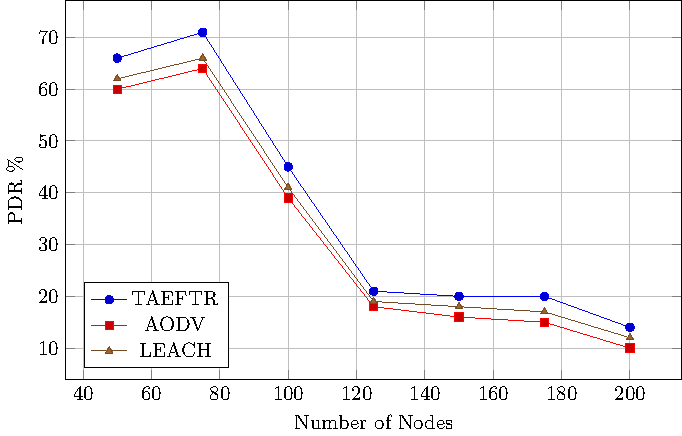
\includegraphics[width=0.48\textwidth]{figures/res1.pdf}
\captionof{figure}{Packet Delivery Ratio versus Number of Nodes}
\label{fig:pdr_nodes}
\end{center}

Figure~\ref{fig:pdr_nodes} presents the packet delivery ratio comparison under varying node density. The proposed TAEFTR protocol achieves consistently higher delivery performance than baseline methods due to adaptive route recovery and failure avoidance. The maximum packet delivery ratio is observed at moderate node density, while performance decreases at higher node counts because of congestion and link contention.


\vspace{0.3cm}

\begin{center}
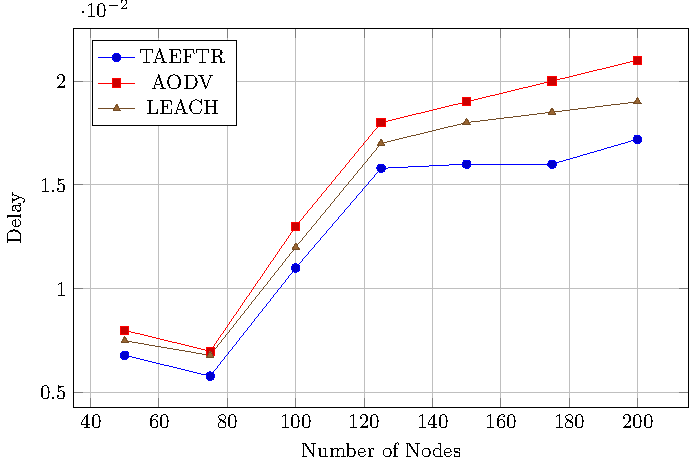
\includegraphics[width=0.48\textwidth]{figures/res2.pdf}
\captionof{figure}{Delay versus Number of Nodes}
\label{fig:delay_nodes}
\end{center}

Figure~\ref{fig:delay_nodes} shows delay comparison under increasing node density. End to end delay rises gradually as the number of nodes increases because routing paths become longer and channel contention increases. However, the proposed method maintains lower delay than conventional protocols through rapid topology adaptation and efficient path selection.



\vspace{0.3cm}

\begin{center}
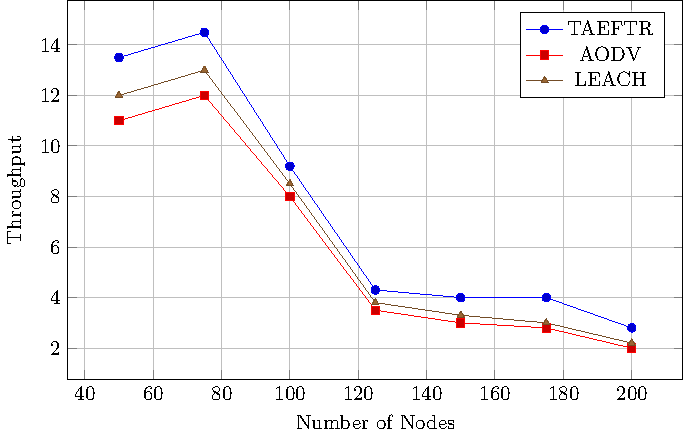
\includegraphics[width=0.48\textwidth]{figures/res3.pdf}
\captionof{figure}{Throughput versus Number of Nodes}
\label{fig:thr_nodes}
\end{center}

Figure~\ref{fig:thr_nodes} illustrates throughput comparison under increasing node density. The proposed routing approach achieves higher throughput because packet loss is minimized and alternative routes are selected immediately after node failure. Throughput reduces at larger node counts due to heavy traffic load.


\vspace{0.3cm}

\begin{center}
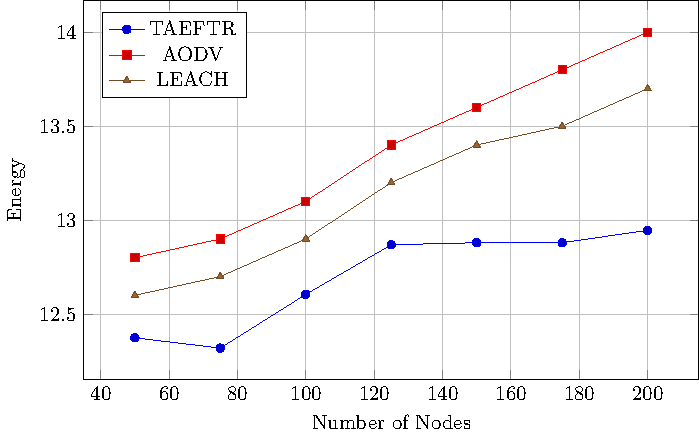
\includegraphics[width=0.48\textwidth]{figures/res4.pdf}
\captionof{figure}{Energy Consumption versus Number of Nodes}
\label{fig:energy_nodes}
\end{center}

Figure~\ref{fig:energy_nodes} presents energy usage comparison among routing methods. The proposed TAEFTR protocol consumes lower energy because forwarding decisions consider residual energy and balanced traffic distribution. This helps in extending the overall operational lifetime of the network.


\vspace{0.3cm}

\begin{center}
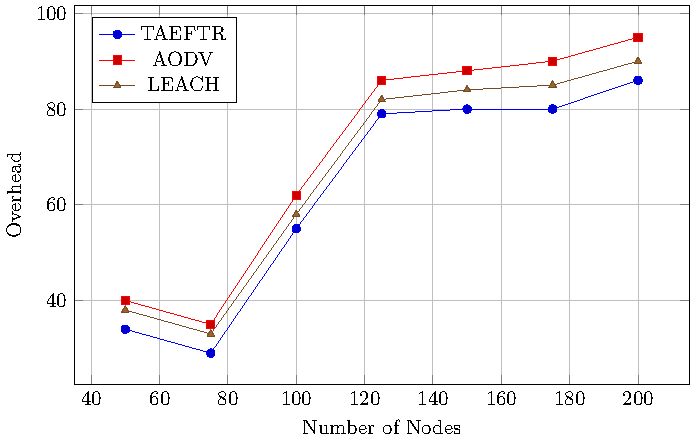
\includegraphics[width=0.48\textwidth]{figures/res5.pdf}
\captionof{figure}{Routing Overhead versus Number of Nodes}
\label{fig:over_nodes}
\end{center}

Figure~\ref{fig:over_nodes} shows routing overhead under varying node density. Control overhead increases with node count because more route updates are required. Even under dense deployment, the proposed method limits unnecessary control messages through efficient route maintenance.

\vspace{0.3cm}

\begin{center}
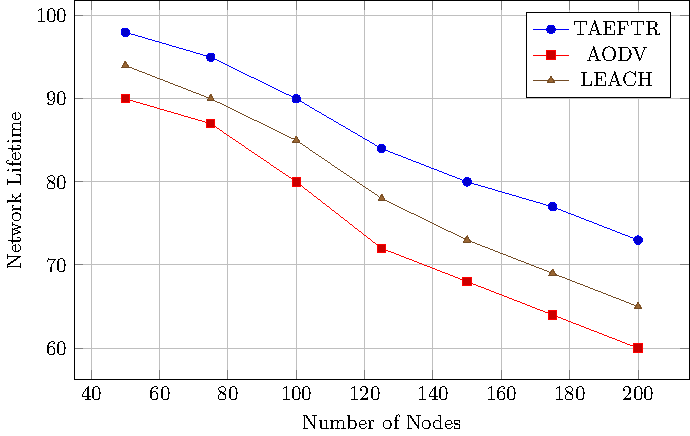
\includegraphics[width=0.48\textwidth]{figures/res6.pdf}
\captionof{figure}{Network Lifetime versus Number of Nodes}
\label{fig:life_nodes}
\end{center}

Figure~\ref{fig:life_nodes} illustrates network lifetime comparison. Because of energy-aware routing and load balancing, the proposed method keeps sensor nodes active for a longer duration. This improves network stability and data collection efficiency.


%=========================================================
\subsection{Traffic Load Based Analysis}

\begin{center}
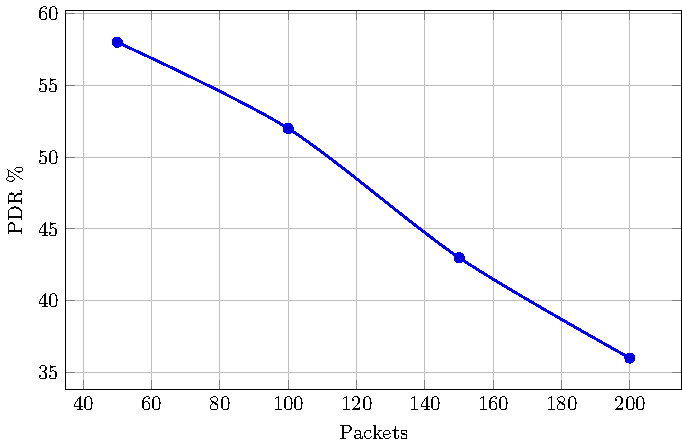
\includegraphics[width=0.48\textwidth]{figures/res7.pdf}
\captionof{figure}{Packet Delivery Ratio versus Packets}
\label{fig:pdr_packets}
\end{center}

Figure~\ref{fig:pdr_packets} shows packet delivery ratio under traffic load variation. As packet generation rate increases, congestion and queue overflow reduce delivery ratio. However, the proposed protocol maintains reliable communication under moderate traffic conditions.


\vspace{0.3cm}

\begin{center}
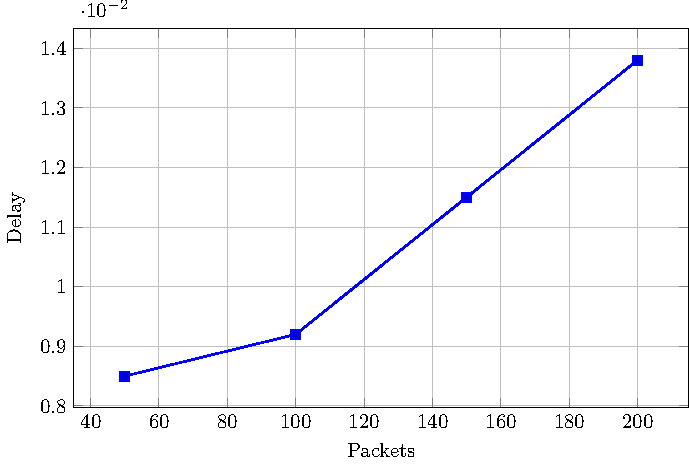
\includegraphics[width=0.48\textwidth]{figures/res8.pdf}
\captionof{figure}{Delay versus Packets}
\label{fig:delay_packets}
\end{center}

Figure~\ref{fig:delay_packets}  presents delay variation under packet load. Delay increases gradually as more packets are injected into the network because waiting time in queues and retransmissions become higher.



\vspace{0.3cm}

\begin{center}
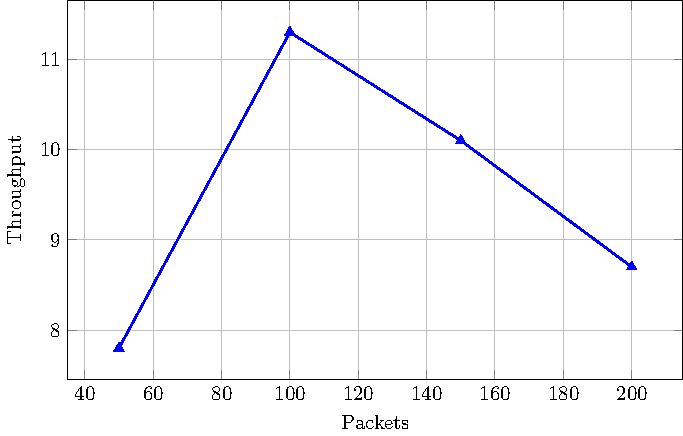
\includegraphics[width=0.48\textwidth]{figures/res9.pdf}
\captionof{figure}{Throughput versus Packets}
\label{fig:thr_packets}
\end{center}

Figure~\ref{fig:thr_packets} illustrates throughput under packet generation load. Throughput initially increases with traffic load as channel utilization improves, then decreases under excessive load due to congestion and collisions.

\vspace{0.3cm}

\begin{center}
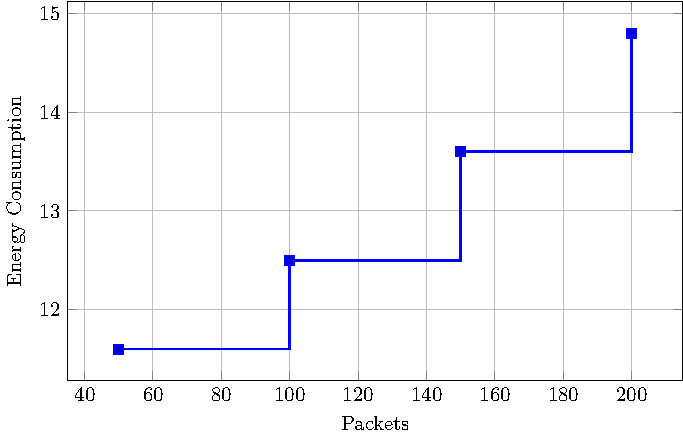
\includegraphics[width=0.48\textwidth]{figures/res10.pdf}
\captionof{figure}{Energy Consumption versus Packets}
\label{fig:energy_packets}
\end{center}

Figure~\ref{fig:energy_packets} shows energy consumption under packet load variation. Higher traffic generates more forwarding and retransmission operations, which increases total energy expenditure across the network.


%=========================================================
\subsection{Additional Performance Metrics}

\begin{center}
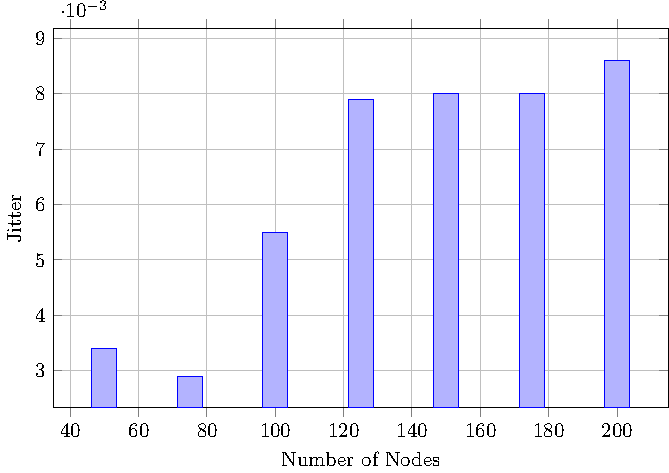
\includegraphics[width=0.48\textwidth]{figures/res11.pdf}
\captionof{figure}{Jitter versus Number of Nodes}
\label{fig:jitter_nodes}
\end{center}

Figure~\ref{fig:jitter_nodes} presents jitter variation under increasing node density. Jitter increases when route changes and medium access contention become frequent. Lower jitter values indicate more stable packet delivery timing.


\vspace{0.3cm}

\begin{center}
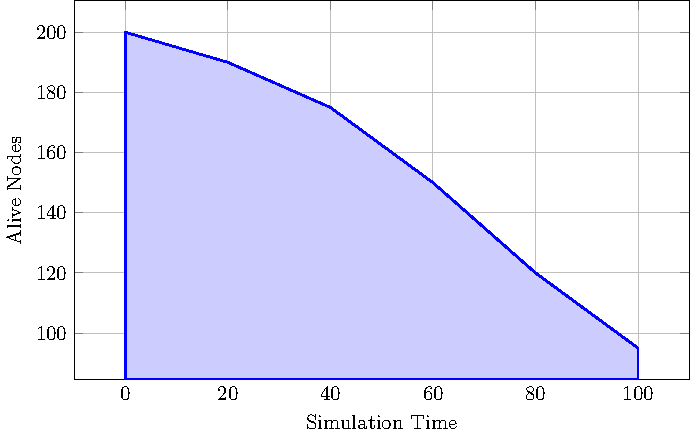
\includegraphics[width=0.48\textwidth]{figures/res12.pdf}
\captionof{figure}{Alive Nodes versus Simulation Time}
\label{fig:alive_time}
\end{center}

Figure~\ref{fig:alive_time}  illustrates active node count over simulation time. The number of alive nodes decreases gradually as energy is consumed during sensing and communication. The proposed protocol maintains more active nodes through balanced energy utilization and efficient routing.
%=========================================================
\section{Conclusion and Future Work}

This work presented the Topology Adaptive Energy Aware Fault Tolerant Routing protocol for improving reliability and efficiency in large scale wireless sensor networks. The proposed method was developed to address common challenges such as node failure, energy depletion, congestion, route instability, and performance degradation under increasing network size. By combining residual energy, communication distance, link quality, and traffic load in the routing decision process, the protocol selects more reliable and energy efficient forwarding paths.

Simulation based evaluation was carried out in the ns3 environment using AODV as the baseline routing framework. The obtained results showed that packet delivery ratio and throughput decrease as node density increases, while delay, jitter, and routing overhead rise because of congestion and frequent route changes. Even under these challenging conditions, the proposed adaptive routing mechanism maintained better communication stability through rapid rerouting and balanced traffic distribution. Energy aware forwarding also reduced unnecessary node exhaustion and improved the operational lifetime of the network.

Overall, the proposed TAEFTR protocol demonstrated effective topology adaptation, improved fault tolerance, and better resource utilization for dynamic wireless sensor networks. Future work can focus on real time deployment, security enhancement, mobility support, and integration of machine learning techniques for predictive failure detection and intelligent routing optimization.

\section*{Declarations}
\subsection*{Ethical Approval}
This manuscript reports studies that do not involve human participants, human data, human tissue, or animals.

\subsection*{Conflict of Interest}
The authors have no conflict of interest to declare that are relevant to the content of this article.

\subsection*{Authors' Contributions}
S. Gopikrishnan contributed to the conceptualization, Formal analysis, drafting the original manuscript, and designing the experimental protocols. Author-2 was responsible for Conceptualization, methodology, software implementation, and dataset curation. Author3 contributed to conceptualization, supervision, and in-depth analysis of the experimental results. Author-3 handled the review and editing of the final draft, as well as the overall validation of the study results.


\subsection*{Funding}
The authors did not receive financial support from any organization for the submitted work.

\subsection*{Availability of data and materials}
Data sharing is not applicable to this article, as no new data were created or analyzed in this study.

\subsection*{Acknowledgment}
We acknowledge that the hardware utilized in this research for evaluation is a part of the Intel IoT Center for Excellence, VIT-AP University. 

\bibliographystyle{cas-model2-names}
\bibliography{references}


\end{document}

